\documentclass[main.tex]{subfiles}
\begin{document}
\newpage
\section{Theoretische Grundlagen}

In diesem Abschnitt werden die theoretischen Grundlagen, die diese Arbeit benötigt, erläutert.

\subsection{Heisenberg Modell}

Um das System von mehreren magnetischen Momenten zu beschreiben, wird das klassische Heisenberg Modell verwendet. Es beschreibt die Wechselwirkung zwischen den magnetischen Momenten der einzelnen Atome.

Die magnetischen Momente \(\vec{\mu}\) werden als klassische dreidimensionale Vektoren der Länge \(\mu_{\text{S}}\) angenommen.
Die normierten und dimensionslosen magnetischen Momente werden mit \(\vec{S}\) bezeichnet:

\begin{align}
	\vec{S}_i = \frac{\vec{\mu}_i}{\mu_{\text{S},i}}
\end{align}

% Da ein Antiferromagnet betrachtet wird, bei dem die magnetischen Momente in
% entgegengesetzte Richtungen zeigen und die Beträge der magnetischen Momente
% gleich sind gilt zusätzlich \(\mu_{\text{S},i} = \mu_{\text{S},j} = \mu_{S}\).

Diese Wechselwirkungen werden durch die Hamiltonfunktion beschrieben, welche sich aus mehreren Komponenten zusammensetzt:

\subsubsection*{Heisenberg Austauschwechselwirkung}
% Heisenberg Austauschwechselwirkung

Die Heisenberg Austauschwechselwirkung beschreibt die Wechselwirkung zwischen den magnetischen Momenten der einzelnen Atome aufgrund von überlappten Wellenfunktionen~\cite{Heisenberg-Ferromagnetismus}. 
Sie ist in der Regel die dominierende Wechselwirkung in magnetisch geordneten Strukturen.
% Klassisch ist sie proportional zum Skalarprodukt der magnetischen Momente:

Eine Herleitung dazu lässt sich in \cite{magnetism-in-condensed-matter} finden.
Die Hamiltonfunktion für die Heisenberg Austauschwechselwirkung kann wie folgt geschrieben werden:

\begin{align}
	\mathcal{H}_{\text{EXC}} = -\sum_{i,j} J_{ij} \vec{S}_i \cdot
	\vec{S}_j\label{eq:hamilton-heisenberg-exc}
\end{align}

\subsubsection*{Dzyaloshinskii-Moriya Wechselwirkung}
% Dzyaloshinskii-Moriya interaction 

Die Dzyaloshinskii-Moriya Wechselwirkung (DMI) beschreibt die indirekte antisymmetrische Interaktion von zwei Spins. Heißt wenn zwei Spins sich eigentlich parallel oder antiparallel ordnen würden, sorgt die DMI dafür, dass die Spins leicht zueinander verkanten. Dadurch entsteht bei schwachen Antiferromagneten die ferromagnetische Komponente~\cite{DMI}.
Sie ist hier die zweitstärkste Wechselwirkung und ist proportional zum Kreuzprodukt der magnetischen Momente:

\begin{align}
	\mathcal{H}_{\text{DMI}} = -\sum_{i,j} \vec{D}_{ij} \cdot (\vec{S}_i
	\times
	\vec{S}_j)\label{eq:hamilton-dmi}
\end{align}

\todo{Herkunft der DMI (Spin-Bahn Kopplung)}
\todo{Kombi Austausch und DMI}

\subsubsection*{Magnetische Anisotropien}
Magnetische Momente können eine Präferenz für eine bestimmte Richtung haben.
% Die Energie, die aufgewendet werden muss, um das magnetische Moment aus dieser Richtung zu drehen, wird als Anisotropie bezeichnet. 
Es gibt verschiedene Arten von Anisotropien.
Die hier betrachteten Anisotropien sind verschiedene kristalline Anisotropien.
Die Anisotropien entstehen also aufgrund der Kristallgitterstruktur. 

Eine Kristall-Anistotropie zweiter Ordnung trägt folgenden Term zur Hamiltonfunktion bei:
\begin{align}
	\mathcal{H}_{\text{2.AI}} = -\sum_{i} \qty(\vec{S}_i)^\dagger
	\mat{d}_i
	\vec{S}_i\label{eq:hamilton-2a}
\end{align}

Bei Anisotropien gibt es immer eine energetisch ungünstige \enquote{schwere} Raumachse und eine günstige \enquote{leichte} Achse, in die sich das System auszurichten versucht.

Ein weiterer Term, der zur Hamiltonfunktion beiträgt, ist die kubische Anisotropie, welche eine Anisotropie vierter Ordnung ist~\cite{GrossMarx}:
\begin{align}
	\mathcal{H}_{\text{4.AI}} = -\sum_{i} L_{i,x} \qty(\vec{S}_{i,y})^2 \qty(\vec{S}_{i,z})^2 
	+ L_{i,y} \qty(\vec{S}_{i,z})^2 \qty(\vec{S}_{i,x})^2 
	+ L_{i,z} \qty(\vec{S}_{i,x})^2 \qty(\vec{S}_{i,y})^2\label{eq:hamilton-4a}
\end{align}

Außerdem wird noch die Zwei-Ionen Anisotropie berücksichtigt:
\begin{align}
	\mathcal{H}_{\text{TIA}} = -\sum_{i,j} \vec{S}_i \mat{\kappa}_{ij} \vec{S}_j\label{eq:hamilton-tia}
\end{align}
\subsubsection*{Zeeman Wechselwirkung}
% Zeeman
Bei einem äußeren Magnetfeld \(B_\text{ext}\) wirkt auf jedes magnetische Moment die Zeeman Wechselwirkung:

\begin{align}
	\mathcal{H}_{\text{Z}} = - B_\text{ext} \sum_{i} \vec{\mu}_i = 
	- B_\text{ext} \sum_{i} \mu_{\text{S},i} \cdot \vec{S}_i\label{eq:hamilton-zeeman}
\end{align}

Diese Wechselwirkung sorgt für eine parallele Ausrichtung aller Spins.

% Dipol Dipol wechselwirkung
\subsubsection*{Dipol-Dipol Wechselwirkung}

Jedes magnetische Moment erzeugt ein Magnetfeld, welches aus hinreichender
Entfernung stehts wie ein Dipolfeld aussieht~\cite{Nolting-3-elektrodynamik}:

\begin{align}
	\vec{B}(\vec{r}) & = \frac{\mu_0}{4\pi} \qty[3 \frac{\vec{r}(\vec{\mu} \cdot
			\vec{r})}{r^5} - \frac{\vec{\mu}}{r^3}]\label{eq:dipolmoment}
\end{align}

Wenn zwei magnetische Momente \(\vec{\mu}_i\) und \(\vec{\mu}_j\) in einem Abstand \(r_{ij}\) zueinander stehen, wirkt auf das magnetische Moment \(\vec{\mu}_i\) das Magnetfeld \(\vec{B}_j\) und auf das magnetische Moment \(\vec{\mu}_j\) das Magnetfeld \(\vec{B}_i\).

% Die Wechselwirkungsenergie zwischen den beiden magnetischen Momenten ist die Energie, die aufgewendet werden muss, um die beiden magnetischen Momente aus dem Magnetfeld des jeweils anderen zu entfernen. Die Wechselwirkungsenergie ist also proportional zum Skalarprodukt der beiden Magnetfelder:

\begin{align}
	\mathcal{H}_{\text{DD}} 
	& = \sum_{i,j} \vec{\mu}_i \cdot \vec{B}_j(\vec{r}_{ij}) \nonumber \\
	& = \sum_{i,j} \frac{\mu_0}{4\pi}
	\cdot \frac{3(\vec{\mu}_i \cdot \vec{r}_{ij})(\vec{\mu}_j \cdot \vec{r}_{ij})
	- \vec{\mu}_i \cdot \vec{\mu}_j \cdot r_{ij}^2}{r_{ij}^5} \nonumber \\
	& = \sum_{i,j} \frac{\mu_0 \cdot \mu_{\text{S,i}} \cdot \mu_{\text{S,j}}}{4\pi}
	\cdot \frac{3(\vec{S}_i \cdot \vec{r}_{ij})(\vec{S}_j \cdot \vec{r}_{ij})
	- \vec{S}_i \cdot \vec{S}_j \cdot r_{ij}^2}{r_{ij}^5}\label{eq:hamilton-dd}
\end{align}

\subsubsection*{Gesamte Hamiltonfunktion}

Die Gesamte Hamiltonfunktion setzt sich aus den einzelnen Komponenten zusammen:

\begin{align}
	\mathcal{H} & = \mathcal{H}_{\text{EXC}} + \mathcal{H}_{\text{DMI}} +
	\mathcal{H}_{\text{2.AI}} + \mathcal{H}_{\text{4.AI}} +
	\mathcal{H}_{\text{TIA}} + \mathcal{H}_{\text{Z}} +
	\mathcal{H}_{\text{DD}}\label{eq:hamilton}\nonumber \\
	& = \underbrace{-\sum_{i,j} J_{ij} \vec{S}_i \cdot \vec{S}_j}_\text{Heisenberg Austausch} % Heisenberg
	\quad \underbrace{-\sum_{i,j} \vec{D}_{ij} \cdot (\vec{S}_i \times \vec{S}_j)}_\text{DMI} % DMI
	\quad \underbrace{-\sum_{i} \qty(\vec{S}_i)^\dagger \mat{d}_i \vec{S}_i}_\text{2. Ordnung Anisotropie}\nonumber  \\ % 2.AI
	& \underbrace{-\sum_{i} L_{i,x} \qty(\vec{S}_{i,y})^2 \qty(\vec{S}_{i,z})^2 + L_{i,y} \qty(\vec{S}_{i,z})^2 \qty(\vec{S}_{i,x})^2 + L_{i,z} \qty(\vec{S}_{i,x})^2 \qty(\vec{S}_{i,y})^2}_\text{4. Ordnung Anisotropie} \nonumber\\ % 4.AI
	& \underbrace{-\sum_{i,j} \vec{S}_i \mat{\kappa}_{ij} \vec{S}_j}_\text{TIA}% TIA
	\quad \underbrace{- B_\text{ext} \sum_{i} \vec{\mu}_i}_\text{Zeeman} \nonumber\\ % Zeeman
	& \underbrace{ + \sum_{i,j} \frac{\mu_0 \cdot \mu_{\text{S,i}} \cdot \mu_{\text{S,j}}}{4\pi} \cdot \frac{3(\vec{S}_i \cdot \vec{r}_{ij})(\vec{S}_j \cdot \vec{r}_{ij}) - \vec{S}_i \cdot \vec{S}_j \cdot r_{ij}^2}{r_{ij}^5}}_\text{Dipol Dipol Wechselwirkung} % DD
\end{align}

\subsection{Bewegungsgleichung: Landau-Lifschitz-Gilbert Gleichung}
% Landau-Lifschitz Gleichung (1935)
Um die Bewegung der magnetischen Momente zu beschreiben, muss aus der Hamiltonfunktion die Bewegungsgleichung abgeleitet werden.

Obwohl die Hamiltonfunktion klassisch ist\todo{klassisches Heisenberg Modell}, kann die Bewegungsgleichung über die Quantenmechanik hergeleitet werden. 
Das Ehrenfest-Theorem besagt, dass die zeitliche Änderung des Erwartungswertes eines Operators gleich dem Erwartungswert des Kommutators des Operators mit der Hamiltonfunktion ist \cite{qm-1-Schwabl}:

\begin{align}
	\dv{\expval{\hat{\vec{S}}_i}}{t} = \frac{1}{i\hbar}
	\expval{\qty[\hat{\vec{S}}_i,
			\hat{\mathcal{H}}]} + \expval{\pdv{\hat{\vec{S}}_i}{t}}
\end{align}

% \begin{align}
% 	\dv{\hat{\vec{S}}_i}{t} = \frac{i}{\hbar} \expval{\qty[\hat{\vec{S}}_i,
% 			\hat{\mathcal{H}}]}
% \end{align}

Mit der Relation 
\(\hat{\vec{S}}_i = \frac{\gamma_i}{\mu_{\text{S}}}\hat{\vec{J}}_i\) 
und der Kommutatorrelation 
\(\qty[\hat{\vec{J}}_i, \hat{\vec{J}}_j] = i \hbar \cdot \varepsilon_{abc} \hat{\vec{J}}_{c,i}\) 
(wobei \(\varepsilon\) das Levi-Civita Symbol und \(\hat{\vec{J}}\) der Drehimpuls ist) ergibt sich:

\begin{align}
	\dv{\vec{S}_i}{t}
	& = -\frac{\gamma}{\mu_{\text{S}}}
	\qty(\vec{S}_i \times \vec{\mathcal{H}}_{\text{i}})\\
	\text{mit} \quad \vec{\mathcal{H}}_{\text{i}} 
	& = - \pdv{\mathcal{H}}{\vec{S}_i}
\end{align}

% \begin{align}
% 	\dv{\vec{S}_i}{t}                             & = -\frac{\gamma
% 	}{\mu_{\text{S}}}
% 	\qty(\vec{S}_i \times
% 	\vec{\mathcal{H}}_{\text{i}}) 
% 	+ \frac{\gamma
% 	}{\mu_{\text{S}}}\vec{S}_i \times
% 	\qty(\vec{S}_i \times \vec{\mathcal{H}}_{\text{i}})
% 	\label{eq:landau-lifschitz}
% \end{align}\cite{landau-lifshitz}

Zusätzlich enthält die Gleichung noch einen Dämpfungsterm~\cite{Gilbert-damping}:

\begin{align}
	\dv{\vec{S}_i}{t} & = -\frac{\gamma }{\mu_{\text{S}}}\qty(\vec{S}_i \times \vec{\mathcal{H}}_{\text{i}}) 
	+ \alpha \qty(\vec{S}_i \times \dv{\vec{S}_i}{t})
\end{align}

Um davon auf eine klassische explizite Bewegungsgleichung zu kommen, muss die
Gleichung zuerst in sich selbst eingesetzt werden:
\begin{align}
	\dv{\vec{S}_i}{t} & = -\frac{\gamma }{\mu_{\text{S}}}\qty(\vec{S}_i
	\times
	\vec{\mathcal{H}}_{\text{i}}) + \alpha \qty(\vec{S}_i \times
	\qty(-\frac{\gamma }{\mu_{\text{S}}}\qty(\vec{S}_i
		\times
		\vec{\mathcal{H}}_{\text{i}}) + \alpha \qty(\vec{S}_i \times
	\dv{\vec{S}_i}{t})))                                                \\
	                  & = -\frac{\gamma }{\mu_{\text{S}}}\qty(\vec{S}_i
	\times
	\vec{\mathcal{H}}_{\text{i}}) - \frac{\alpha\gamma}{\mu_\text{S}}
	\qty(\vec{S}_i \times \qty(\vec{S}_i \times
		\vec{\mathcal{H}}_{\text{i}})) +
	\alpha^2 \qty(\vec{S}_i \times \qty(\vec{S}_i \times
		\dv{\vec{S}_i}{t}))
\end{align}
Aufgrund der Identitäten \(\vec{a} \times \qty(\vec{b} \times \vec{c}) =
\vec{b} \qty(\vec{a} \cdot \vec{c}) - \vec{c} \qty(\vec{a} \cdot \vec{b})\),
\(\vec{S}_i \bot \dv{\vec{S}_i}{t}\) und \(\vec{S}_i \cdot \vec{S}_i = 1\)
ergibt sich:
\begin{align}
	\alpha^2 \qty(\vec{S}_i \times \qty(\vec{S}_i \times
	\dv{\vec{S}_i}{t})) & = -\alpha^2\dv{\vec{S}_i}{t}
\end{align}
Somit lässt sich die Bewegungsgleichung nach \(\dv{\vec{S}_i}{t}\) auflösen.
Damit ergibt sich die Landau-Lifschitz-Gilbert Gleichung:
\todo{fascinating world of the LLG equation}
\begin{align}
	\dv{\vec{S}_i}{t} & = -\frac{\gamma
	}{\mu_{\text{S}}(1+\alpha^2)}\qty[\underbrace{\vec{S}_i \times
			\vec{\mathcal{H}}_{\text{i}}}_\text{Präzession} +
		\underbrace{\alpha \vec{S}_i
			\times
			\qty(\vec{S}_i \times
			\vec{\mathcal{H}}_{\text{i}})}_\text{Dämpfung}]\label{eq:llg}
\end{align}
% \todo{erklärung der einzelnen Terme}
% Beim Vergleich mit der Landau-Lifschitz-Gleichung \eqref{eq:landau-lifschitz} fällt auf, dass sich einerseits der vorfaktor geändert hat und andererseits ein Dämpfungsterm hinzugekommen ist. Für \(\alpha = 0\) sind die Gleichungen identisch. 

Die Landau-Lifschitz-Gilbert Gleichung unterscheidet sich nur über die Faktoren
(\(\frac{1
}{1 + \alpha^2}\) und \(\alpha\)) von der Landau-Lifschitz Gleichung

Der Präzessionsterm beschreibt die Präzession der magnetischen Momente um das effektive Feld.

% Der Dämpfungsterm beschreibt die Energie, die aufgewendet werden muss, um die magnetischen Momente zu drehen. 
Der Dämpfungsterm ist eine Art Reibungsterm, der die Präzession der magnetischen Momente dämpft und für eine Relaxion in Richtung des effektiven Feldes sorgt.

Bis jetzt wurde das System nur bei \(T = \qnt{0}{\kelvin}\) betrachtet.
% Was jetzt noch fehlt ist das weiße Rauschen von \( \vec{\mathcal{H}}_i \), welches durch die endliche Temperatur entsteht. 
Durch addition eines Rauschterms \(\vec{\xi}_i(t)\) kann die Bewegungsgleichung auch für endliche Temperaturen beschrieben werden.
% Dieses wird durch einen stochastischen Term \(\vec{\xi}_i(t)\) beschrieben, der die Bewegungsgleichung zu einer stochastischen Differentialgleichung macht:
Dabei handelt es sich um ein Gausssches weißes Rauschen, welches unkorreliert in Raum und Zeit ist.

\todo{Langevin Dynamik}
\begin{align}
	\vec{\mathcal{H}}_{\text{i}} 
	& = -\pdv{\mathcal{H}}{\vec{S}_i} + \vec{\xi}_i(t) \\
	\expval{\vec{\xi}_i(t)} & = 0 \\
	\expval{\xi_{i,\alpha}(t) \xi_{j,\beta}(t')} 
	& = \frac{2\mu_\text{S} \alpha}{\gamma}k_\text{B} T \cdot \delta_{ij} \delta_{\alpha \beta}	\delta(t-t')
\end{align}

\begin{figure}[H]
	\centering
	\subcaptionbox{\(T = \qnt{0}{\kelvin} \)}{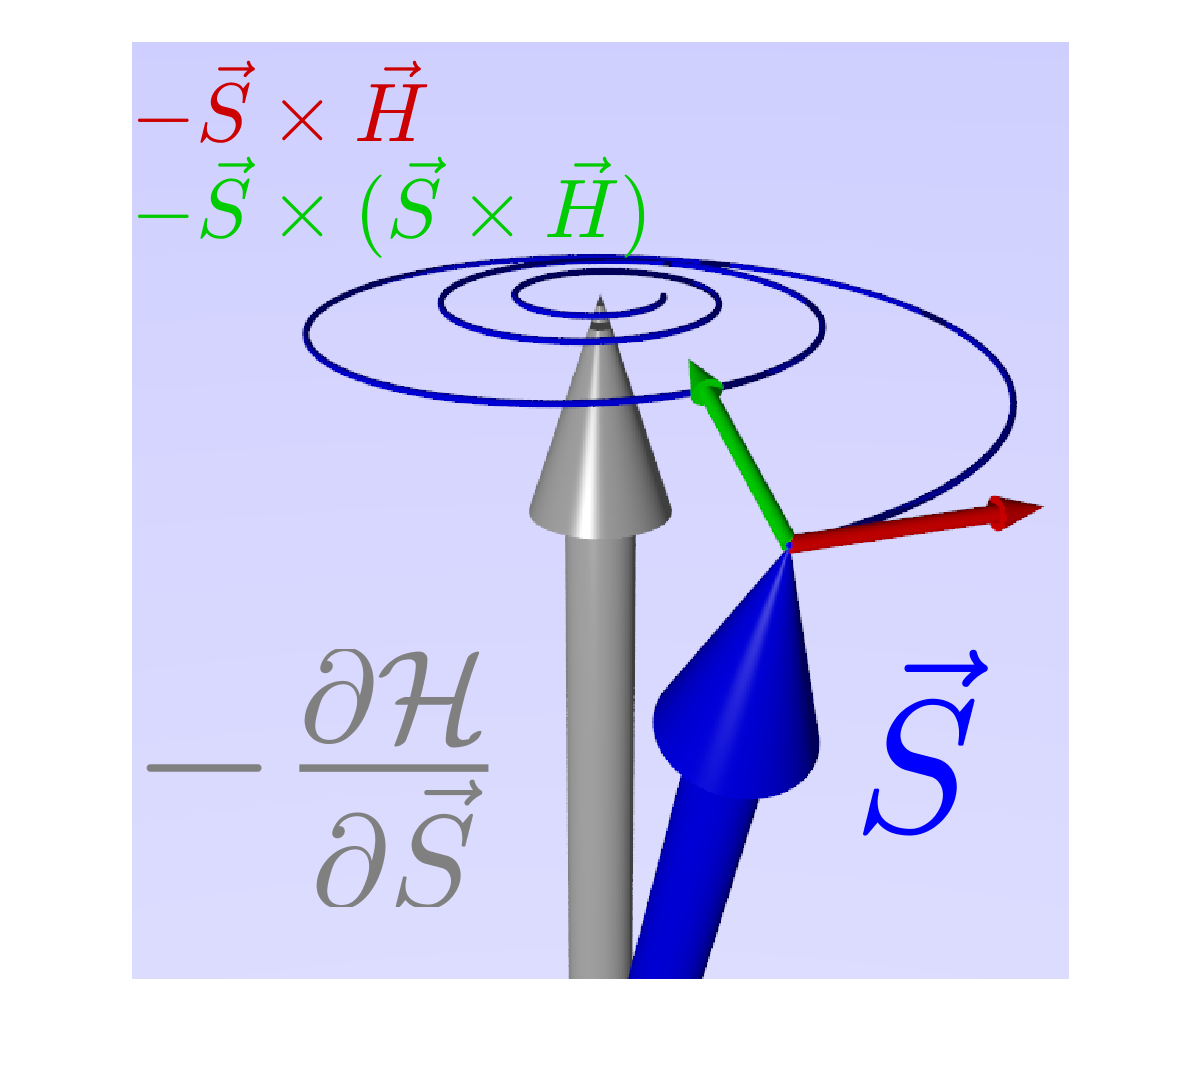
\includegraphics[width=0.45\textwidth]{bilder/jschlege/LLG_T0_labeled.png}}
	\subcaptionbox{\(T \gg \qnt{0}{\kelvin} \)}{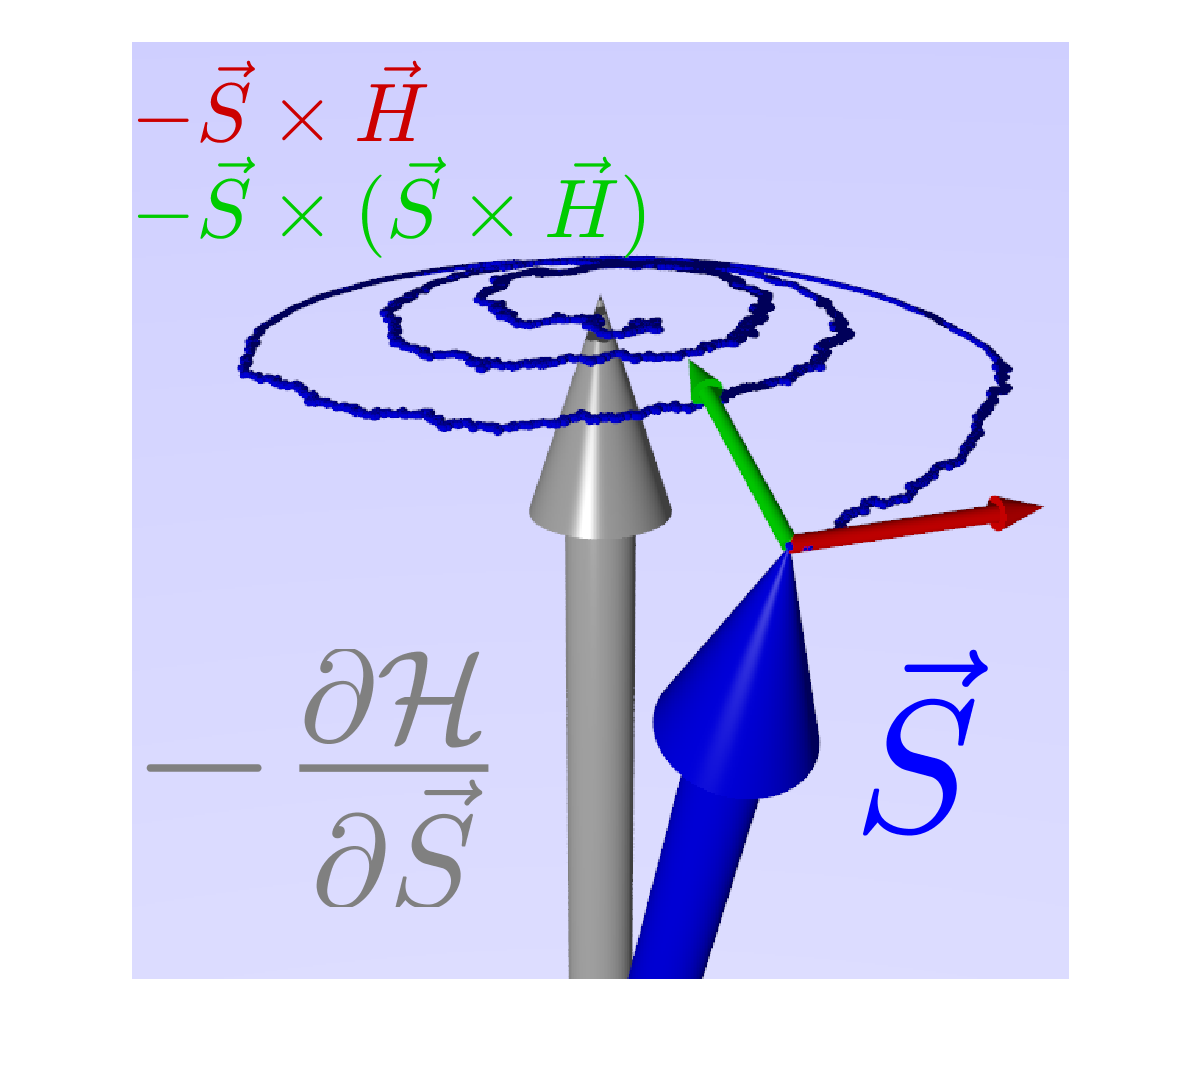
\includegraphics[width=0.45\textwidth]{bilder/jschlege/LLG_labeled.png}}
	\caption{Visualisierung der LLG-Gleichung. Der blaue Vektor entspricht dem Spin \(\vec{S}\) und die blaue Linie ist die Dynamik. Der Graue Vektor entspricht dem effektiven Feld, ohne Rauschen. Der Ptäzessionsterm wird durch den roten Vektor beschrieben und der Dämpfungsterm durch den grünen.~\cite{schlegel-master}}
	\label{fig:llg-rauschen}
\end{figure}

\subsection{Modellierung von Orthoferrit}

Orthoferrite sind chemische Verbindungen der Form \ce{RFeO3}, wobei \ce{R} ein Rest ist, durch den sich die verschiedenen Orthoferrite unterscheiden. Hier bildet Erbium (\ce{Er}) diese Restgruppe. 
\todo{Samarium jetzt oder erst	später?}

% \begin{figure}[htbp]
% 	\centering
% 	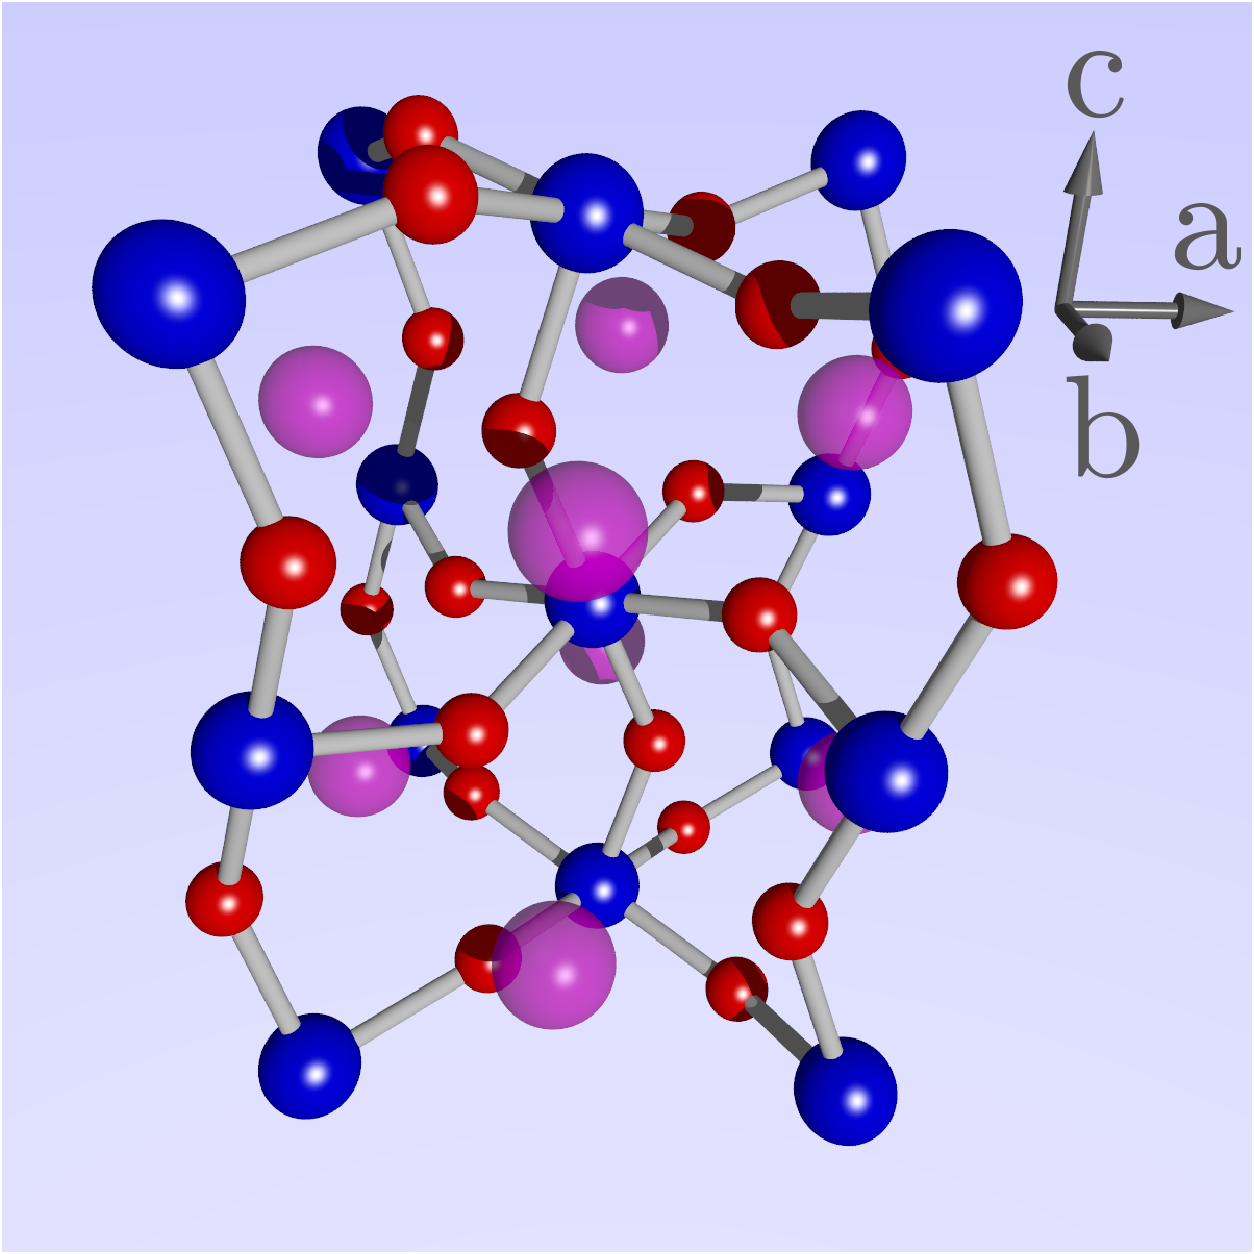
\includegraphics[width=0.4\textwidth]{bilder/jschlege/UnitCell_labeled.png}
% 	\caption{Kristallstruktur von
% 		\ce{ErFeO3}. Die Eisenatome sind dabei blau, die
% 		Sauerstoffatome rot und die Erbiumatome magenta gefärbt.
% 		\cite{schlegel-master}}
% 	\label{fig:orthoferrit}
% \end{figure}

% \todo{erklärung für Samarium (reorientierungstemperatur)}

Die Reorientierungstemperatur \(T_l < T < T_h\) liegt bei Erbiumferrit bei ungefähr \qnt{110}{\kelvin}~\cite{Deng2015}. 
Durch teilweises Ersetzen von Erbium durch Samarium kann die Reorientierungstemperatur erhöht werden. Be \ce{Sm_{0.7}Er_{0.3}FeO3} liegt sie ungefähr bei Raumtemperatur, weshalb es im Experiment einfacher zu untersuchen ist~\cite{Fitzky2021}.

% Parameter für Simulation
% \todo{wer hat die Parameter bestimmt?}

Für die Simulation wird ein Modell von einem Orthoferriten verwendet, bei dem
die Anisotropie-Parameter angepasst wurden, um eine Reorientierungstemperatur
bei Raumtemperatur wie bei \ce{Sm_{0.7}Er_{0.3}FeO3} zu erhalten.
Simuliert wird dabei nur das Gitter aus Eisenatomen. Die Einflüsse der
Sauerstoff-, Erbium und Samariumatome steckt in den Anisotropie-Parametern. Die
Einheitszelle ist in \cref{fig:orthoferrit} dargestellt.

Die verwendeten Simulationsparameter sind folgende:

\begin{align}
	J_1           & = \qnt{-22,32}{\milli\electronvolt}, \quad J_2 =
	\qnt{-1,4}{\milli\electronvolt}\label{eq:params-exc}
	\\
	\mat{d}       & = \mqty(
	\num{0.0153}  & \num{-0.0153}                                   & 0
	\\
	\num{-0.0153} & \num{0.0153}                                    & 0
	\\
	0             & 0                                               &
	\num{0.905})\unit{\milli\electronvolt} \label{eq:params-2a}
	\\
	L_x           & = L_y = L_z =
	\qnt{0.036}{\milli\electronvolt}\label{eq:params-4a}
	\\
	\mat{\kappa}  & = \mqty(
	0             & 0                                               & 0
	\\
	0             & 0                                               & 0
	\\
	0             & 0                                               &
	\num{-0.1255})\unit{\milli\electronvolt} \label{eq:params-tia}
	\\
	\vec{D}_x     & = \mqty*(\num{\pm 0.0036}
	\\ \num{\pm 0.1268} \\ \num{\pm
		0.1255})\unit{\milli\electronvolt} , \quad
	\vec{D}_y = \mqty*(\num{\pm 0.1268}
	\\ \num{\pm 0.0036} \\ \num{\pm
		0.1255})\unit{\milli\electronvolt} , \quad
	\vec{D}_z = \mqty*(\num{\pm 0.1038}
	\\ \num{\pm 0.2252} \\ 0)\unit{\milli\electronvolt} \label{eq:params-dmi}
\end{align}

\(J_1\) ist hier der Parameter für die Heisenberg-Austauschwechselwirkung
\eqref{eq:hamilton-heisenberg-exc} mit den nächsten Nachbarn (6) und \(J_2\)
die mit den übernächsten Nachbarn (12). \todo{Antiferromagnetisch?}\(\bm{d}\)
beschreibt die uniaxiale Anisotropie\eqref{eq:hamilton-2a}, \(L_x\), \(L_y\)
und \(L_z\) sind die Koeffizienten der kubischen
Anisotropie\eqref{eq:hamilton-4a}, \(\bm{\kappa}\) ist die Zwei-Ionen
Anisotropie\eqref{eq:hamilton-tia} und \(\vec{D}_x\), \(\vec{D}_y\) und
\(\vec{D}_z\) sind die Dzyaloshinskii-Moriya Vektoren\eqref{eq:hamilton-dmi}.

Die Dipol-Dipol Wechselwirkung\eqref{eq:hamilton-dd} wird in der Simulation
nicht berücksichtigt, da sie im Vergleich zu den anderen Wechselwirkungen
vernachlässigbar ist.

\todo{erklärung Realisation Reorientierungsübergang (Welche Werte werden modifiziert um die Temperatur zu ändern)}

\begin{align}
	\vec{e}_a &= \frac{\vec{e}_x - \vec{e}_y}{\sqrt{2}} \\
	\vec{e}_b &= \frac{\vec{e}_x + \vec{e}_y}{\sqrt{2}} \\
	\vec{e}_c &= \vec{e}_z
\end{align}

\begin{figure}[htbp]
	\centering
	\subcaptionbox{Einheitszelle mit DMI Vektoren(gelb)\label{subfig:orthoferrit-dmi}}{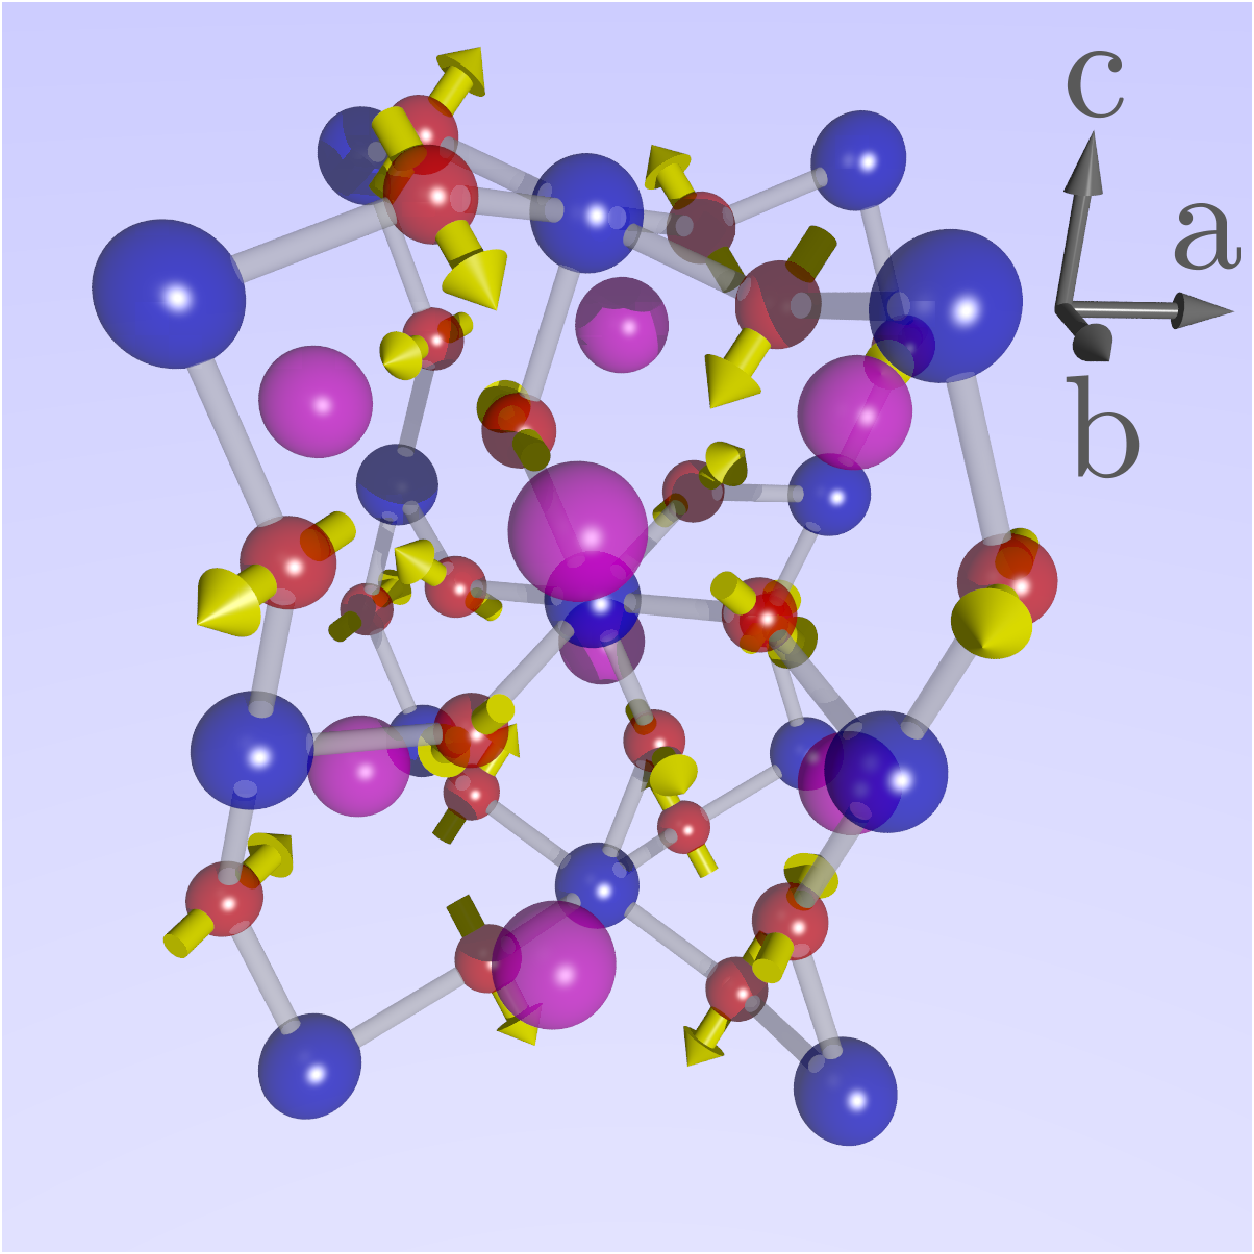
\includegraphics[width=0.3\textwidth]{bilder/jschlege/UnitCell_withDMI_labeled.png}}
	\subcaptionbox{Einheitszelle mit magnetischen Momenten (grün) für \(T<T_l\)\label{subfig:orthoferrit-below-rt}}{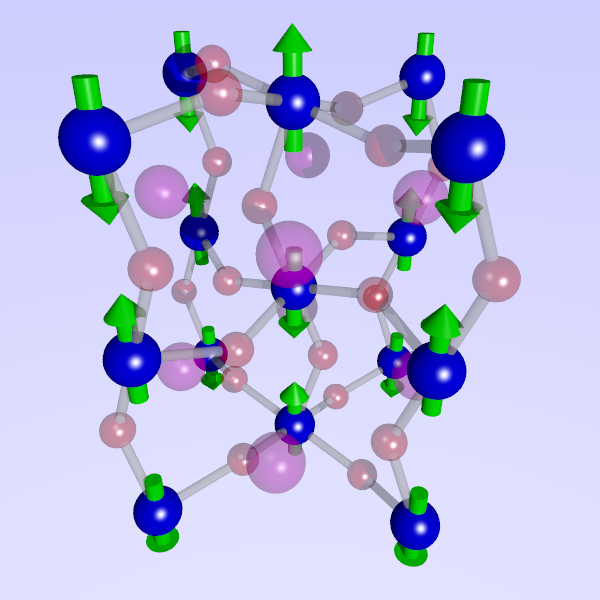
\includegraphics[width=0.3\textwidth]{bilder/jschlege/UnitCell_belowRT.png}}
	\subcaptionbox{Einheitszelle mit magnetischen Momenten (grün) für \(T>T_h\)\label{subfig:orthoferrit-above-rt}}{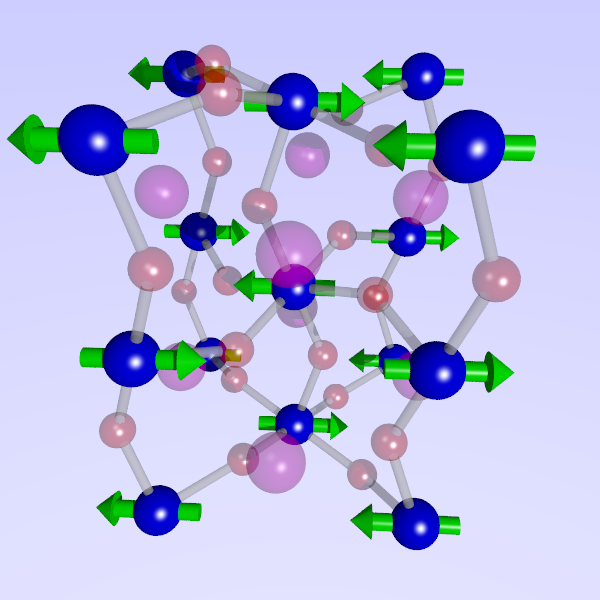
\includegraphics[width=0.3\textwidth]{bilder/jschlege/UnitCell_aboveRT.png}}
	\caption{Kristallstruktur von \ce{ErFeO3}.  Die Eisenatome sind dabei blau, die Sauerstoffatome rot und die Erbiumatome magenta gefärbt. 
	\textbf{(a)} Die DMI Vektoren sind gelb eingezeichnet und die Richtung entspricht den Werten in \cref{eq:params-dmi} 
	\textbf{(b)} Unterhalb der Reorientierungstemperatur dominiert die Anisotropie zweiter Ordnung (\cref{eq:hamilton-2a,eq:params-2a}), weshalb die magnetischen Momente quasi parallel zur c-Achse ausgerichtet sind. 
	\textbf{(c)} Oberhalb der Reorientierungstemperatur dominiert die Zwei-Ionen Anisotropie (\cref{eq:hamilton-tia,eq:params-tia}), weshalb die magnetischen Momente quasi senkrecht zur c-Achse ausgerichtet sind. Die Anisotropie zweiter Ordnung sorgt dafür, dass die magnetischen Momente quasi parallel zur a-Achse ausgerichtet sind.~\cite{schlegel-master}}
	\label{fig:orthoferrit}
\end{figure}

\subsection{Telegrafenrauschen}

\todo{Einleitung warum Telegrafenrauschen relevant ist}

% Das Telegrafenrauschen ist ein stochastischer Prozess, der aus zwei Zuständen besteht, die zufällig zwischen einander wechseln.
\todo{erkllärung TGR (mehrere zustände) übergangszeit deutlich kürzer als
	aufenthaltszeit}

Hier wird ein Telegrafenrauschen mit zwei Zuständen betrachtet.
Ein gängiges Modell ist der Dichtomische Markow-Prozess (DMP).
Die Gleichungen dazu sind aus~\cite{matphys} entnommen.

Dieser entspricht einer Markow-Kette mit zwei Zuständen (\(c_1\) und \(c_2\))
zwischen denen die Zustandsvariable \(X(t)\) zufällig hin und her wechselt. Aus
den Übergangsraten \(\lambda_1\) und \(\lambda_2\) bildet sich die
Übergangsmatrix \(\mathbf{W}\):
\todo{erkllärung Übergangsmatrix + Zitat}
\begin{align}
	\dv{P(t)}{t} & = \mathbf{W} P(t) \\
	\mathbf{W}   & = \mqty(
	-\lambda_1   & \lambda_2         \\
	\lambda_1    & -\lambda_2)
\end{align}

Die Übergangsraten sind umgekehrt proportional zu den mittleren Verweilzeiten
(die mittlere Zeit, die \(X(t)\) in einem Zustand verbringt): \(\lambda_i =
\frac{1}{\tau_i}\).

Mit der mittleren Übergangsrate \(\lambda\) lässt sich die Übergangsmatrix
zeitlich entwickeln:
\begin{align}
	\lambda                            & = \frac{1}{2} \qty(\lambda_1 +
	\lambda_2)
	\\
	e^{\mathbf{W}t}                    & = \frac{1}{2\lambda}
	\mqty(\lambda_2 + \lambda_1
	e^{-2\lambda t}                    & \lambda_2 \qty(1- e^{-2\lambda t})
	\\
	\lambda_1 \qty(1- e^{-2\lambda t}) & \lambda_1 + \lambda_2 e^{-2\lambda
		t})
\end{align}

Für \( \lim_{t \to \infty} \) erhalten wir folgende
Aufenthaltswahrscheinlichkeiten:
\begin{align}
	P(1) & = \frac{\tau_1}{\tau_1 + \tau_2} =
	\frac{\lambda_2 }{\lambda_1 +
		\lambda_2}
	\\
	P(2) & = \frac{\tau_2}{\tau_1 + \tau_2} =
	\frac{\lambda_1 }{\lambda_1 +
		\lambda_2}
\end{align}
Damit lässt sich die gemittelte Zustandsvariable \(\expval{X}\) und die Varianz
\(\expval{\qty(X - \expval{X})^2}\) berechnen:
\begin{align}
	\expval{X}                      & = c_1 P(1) + c_2 P(2) = \frac{\tau_1
		c_1 + \tau_2
		c_2}{\tau_1 + \tau_2} = \frac{\lambda_2 c_1 + \lambda_1
		c_2}{\lambda_1 +
		\lambda_2}
	\\
	\expval{\qty(X - \expval{X})^2} & = \frac{\tau_1 \tau_2
		(c_1-c_2)^2}{(\tau_1 + \tau_2)^2} = \frac{\lambda_1 \lambda_2
		(c_1-c_2)^2}{(\lambda_1 + \lambda_2)^2}
\end{align}
Die Autokorrelationsfunktion und die Korrelationszeit lassen sich damit dann
auch berechnen:
\begin{align}
	\delta X(t)                     & = X(t) - \expval{X}
	\\
	\expval{\delta X(0)\delta X(t)} & = \frac{\lambda_1 \lambda_2
		(c_1-c_2)^2}{(\lambda_1 + \lambda_2)^2} \cdot \exp(-2\lambda t)
	\\
	\tau_\mathrm{corr}              & = \frac{1}{2\lambda} =
	\frac{1}{\lambda_1 +
		\lambda_2} = \frac{\tau_1 \tau_2}{\tau_1 + \tau_2}
\end{align}

\subsubsection*{Symmetrischer DMP}

Wenn \(c_1=-c_2=c\) und \(\lambda_1 = \lambda_2 = \lambda\) gilt, ist der DMP
symmetrisch und viele Ausdrücke vereinfachen sich:
\begin{align}
	\expval{X}        & = 0                     \\
	\expval{X^2}      & = c^2                   \\
	\expval{X(0)X(t)} & = c^2 \exp(-2\lambda t)\label{eq:autokorr-sym-dmp}
\end{align}
\todo{\(e^{-2\lambda t}\) oder \(e^{-\lambda t}\)?}

\subsubsection*{Spektrale Leistungsdichte und Autokovarianz}

Um das Rauschen in der Frequenzdomäne zu betrachten, wird die spektrale
Leistungsdichte \(P(\omega)\) verwendet. Sie lässt sich aus der abgeschnittenen
Fouriertransformierten von \(X(t)\) berechnen:
\begin{align}
	\hat{X}^T(\omega) & = \int_0^T \dif t \ X(t) \exp(-i \omega
	t)
	\\
	P(\omega)         & = \lim_{T \to \infty} \frac{1}{T}
	\abs{\hat{X}^T(\omega)}^2
\end{align}

Die Spektrale Leistungsdichte lässt sich auch aus der Autokovarianz berechnen~\cite{Petroni}:
\begin{align}
	P(\omega) = \int_{-\infty}^{\infty} \dif \tau \ \exp(-i \omega
	\tau) \expval{X(0) X(\tau)}\label{eq:spd}
\end{align}
\todo{inverse Funktion (SPD -> autocov)?}

Eine Herleitung dazu befindet sich in~\cite{Petroni}

Die Spektrale Leistungsdichte für den symmetrischen DMP lässt sich somit
berechnen:

\begin{align}
	P_\text{DMP}(\omega) & = \int_{-\infty}^{\infty} \dif \tau \ e^{-i
			\omega \tau} \expval{X(0)X(\tau)}\nonumber
	\\
	                     & = c^2 \int_{-\infty}^{\infty} \dif \tau \ e^{-i
			\omega
			\tau}e^{-\lambda \abs{\tau}}\nonumber
	\\
	                     & = c^2 \int_{-\infty}^{0} \dif \tau \ e^{-i
			\omega \tau}e^{\lambda
	\tau} + c^2 \int_{0}^{\infty} \dif \tau \ e^{-i \omega \tau}e^{-\lambda
	\tau}\nonumber
	\\
	                     & = c^2 \int_{0}^{\infty} \dif \tau \ e^{-\lambda
			\tau} \qty(e^{i \omega
		\tau} + e^{-i \omega \tau})\nonumber
	\\
	                     & = c^2 \qty[\frac{e^{-\tau(\lambda +
					i\omega)}}{\lambda + i\omega} +
		\frac{e^{-\tau(\lambda - i\omega)}}{\lambda -
			i\omega}]_{0}^{\infty}\nonumber
	\\
	                     & = c^2\qty(\frac{1}{\lambda + i\omega} +
	\frac{1}{\lambda -
		i\omega})\nonumber
	\\
	                     & = \frac{c^2 \cdot 2\lambda}{\lambda^2 +
		\omega^2},
\end{align}
was einer Lorenzverteilung mit dem Maximum bei \(\omega=0\) entspricht.

% bibliography (temporary)
% \bibliography{literatur} \todo{comment out before compiling main.tex}

\end{document}